% !TEX encoding = UTF-8
% !TEX TS-program = pdflatex
% !TEX root = ../tesi.tex

%**************************************************************
\chapter{Analisi dei requisiti}
\label{cap:analisi-requisiti}
%**************************************************************

Questo capitolo descrive i casi d'uso e i requisiti della piattaforma moviORDER, individuati e classificati per definire nel dettaglio obiettivi e funzionalità del sistema. I casi d'uso e i requisiti sono stati dedotti da un'analisi preliminare eseguita dal tutor aziendale, la quale è stata perfezionata dallo stagista per perseguire massima efficienza ed efficacia del sistema. Le convenzioni adottate per il codice univoco di casi d'uso e requisiti sono presenti in Appendice §\ref{}.

\section{Casi d'uso}

Per lo studio dei casi di utilizzo della piattaforma sono stati creati dei diagrammi dei casi d'uso che meglio descrivono funzioni e/o servizi offerti dal sistema, così come sono percepiti e utilizzati dagli attori che interagiscono con il sistema stesso. Per la definizione dei diagrammi UML dei casi d'uso è stato utilizzato lo standard UML 2.0.

\subsection{Attori del sistema}

Lo scopo di moviORDER è permettere alle aziende che forniscono dei prodotti di vendere gli stessi ai propri clienti tramite un'applicazione multipiattaforma. Quindi moviORDER viene distribuita da VISIONEIMPRESA alle aziende che forniscono prodotti, la quale viene distribuita dalle aziende stesse ai propri clienti. Gli utilizzatori finali di moviORDER sono quindi i clienti delle singole aziende che sono clienti di VISIONEIMPRESA.
L'accesso all'applicazione è consentito solamente agli utenti provvisti di credenziali di accesso, le quali vengono distribuite, insieme all'applicazione, dal fornitore. Non è prevista quindi una funzionalità di registrazione. Nel contesto di moviORDER vi sono quindi due tipologie di attori:
\begin{enumerate}
	\item \textbf{Utente non autenticato}: è un utente che non ha effettuato l'accesso al sistema al quale viene offerta la sola funzionalità di autenticazione. Una volta che un utente non autenticato viene riconosciuto accedendo al sistema, diventa un utente autenticato;
	\item \textbf{Utente autenticato}: è un utente che ha effettuato l'accesso al sistema e che può usufruire di tutte le sue funzionalità. Le funzionalità offerte all'utente autenticato sono:
	\begin{itemize}
		\item possibilità di effettuare il logout;
		\item possibilità di aggiungere articoli al proprio carrello;
		\item possibilità di modificare gli articoli nel proprio carrello;
		\item possibilità di rimuovere articoli dal proprio carrello;
		\item possibilità di inviare un ordine alla propria azienda.
	\end{itemize}
\end{enumerate}

\subsection{UC1 - Azioni utente non autenticato}

\begin{figure}[!h] 
    \centering 
    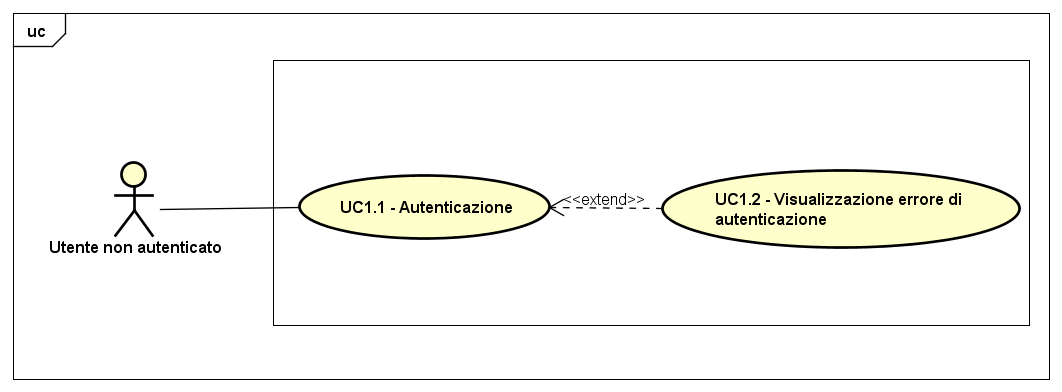
\includegraphics[width=0.9\columnwidth]{usecase/generaleNonAutenticato} 
    \caption{Use Case - UC1: Azioni utente non autenticato}
\end{figure}

\begin{itemize}
	\item \textbf{Attore}: Utente non autenticato;
	\item \textbf{Descrizione}: L'attore può eseguire l'operazione di autenticazione alla piattaforma moviORDER;
	\item \textbf{Pre-condizioni}: L'attore ha avviato l'applicazione e non è ancora stato riconosciuto dal sistema;
	\item \textbf{Post-condizioni}: L'attore ha eseguito l'operazione che desiderava compiere da utente non autenticato;
	\item \textbf{Scenario principale}: UC1.1 - Autenticazione;
	\item \textbf{Scenario alternativo}: L'attore ha fornito credenziali di accesso non corrispondenti a nessun utente registrato dall'azienda, oppure non riesce ad accedere al sistema perché è stato bloccato dall'azienda stessa: UC1.2 - Visualizzazione errore di autenticazione. 
\end{itemize}

\subsection{UC1.1 - Autenticazione}

\begin{figure}[!h] 
    \centering 
    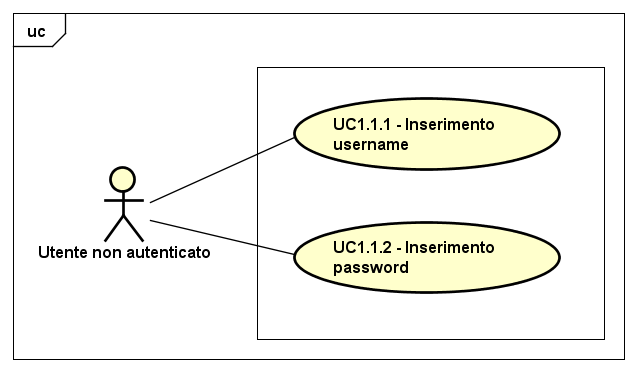
\includegraphics[width=0.9\columnwidth]{usecase/autenticazione} 
    \caption{Use Case - UC1.1: Autenticazione}
\end{figure}

\begin{itemize}
	\item \textbf{Attore}: Utente non autenticato;
	\item \textbf{Descrizione}: L'attore può eseguire l'operazione di autenticazione;
	\item \textbf{Pre-condizioni}: L'attore ha avviato l'applicazione, non è ancora riconosciuto dal sistema e ha espresso la volontà di effettuare l’autenticazione a moviORDER;
	\item \textbf{Post-condizioni}: L'attore ha eseguito l'operazione di accesso al sistema ed è quindi ora riconosciuto come utente autenticato;
	\item \textbf{Scenario principale}: 
		\begin{enumerate}
			\item UC1.1.1 - Inserimento username;
			\item UC1.1.2 - Inserimento password.
		\end{enumerate} 
\end{itemize}

\subsection{UC1.1.1 - Inserimento username}

\begin{itemize}
	\item \textbf{Attore}: Utente non autenticato;
	\item \textbf{Descrizione}: L'attore deve inserire una username per l'operazione di autenticazione;
	\item \textbf{Pre-condizioni}: L'attore ha avviato l'applicazione, non è ancora riconosciuto dal sistema e il sistema richiede l'inserimento di una username per l'operazione di autenticazione;
	\item \textbf{Post-condizioni}: L'attore ha inserito la username per l'operazione di autenticazione;
	\item \textbf{Scenario principale}: L'attore inserisce la username tramite una text box.
\end{itemize}

\subsection{UC1.1.2 - Inserimento password}

\begin{itemize}
	\item \textbf{Attore}: Utente non autenticato;
	\item \textbf{Descrizione}: L'attore deve inserire una password per l'operazione di autenticazione;
	\item \textbf{Pre-condizioni}: L'attore ha avviato l'applicazione, non è ancora riconosciuto dal sistema e il sistema richiede l'inserimento di una password per l'operazione di autenticazione;
	\item \textbf{Post-condizioni}: L'attore ha inserito la password per l'operazione di autenticazione;
	\item \textbf{Scenario principale}: L'attore inserisce la password tramite una text box.
\end{itemize}

\subsection{UC1.2 - Visualizzazione errore di autenticazione}

\begin{itemize}
	\item \textbf{Attore}: Utente non autenticato;
	\item \textbf{Descrizione}: L'attore inserisce credenziali di accesso non corrispondenti a nessun utente registrato dall'azienda, oppure l'utente è stato bloccato dall'azienda stessa;
	\item \textbf{Pre-condizioni}: L'attore ha avviato l'applicazione, non è ancora riconosciuto dal sistema e inserisce credenziali di accesso non corrispondenti a nessun utente registrato dall'azienda, oppure è stato bloccato;
	\item \textbf{Post-condizioni}: L'attore ha visualizzato un messaggio d'errore relativo all'impossibilità di eseguire l'autenticazione per inserimento di credenziali errate o perché è stato bloccato;
	\item \textbf{Scenario principale}: L'attore visualizza un messaggio d'errore relativo all'impossibilità di eseguire l'autenticazione per inserimento di credenziali errate o perché è stato bloccato.
\end{itemize}

\subsection{UC2 - Azioni utente autenticato}

\begin{figure}[!h] 
    \centering 
    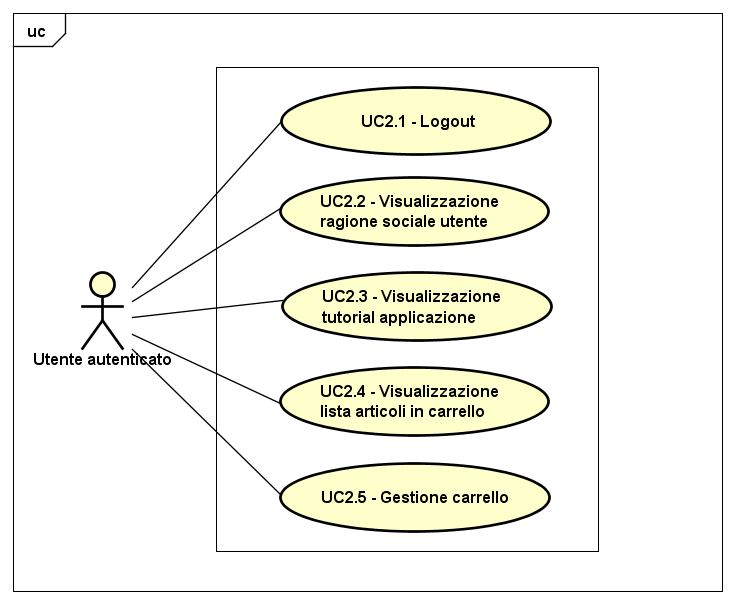
\includegraphics[width=0.9\columnwidth]{usecase/generaleAutenticato} 
    \caption{UC2 - Azioni utente autenticato}
\end{figure}

\begin{itemize}
	\item \textbf{Attore}: Utente autenticato;
	\item \textbf{Descrizione}: L'attore può:
	\begin{enumerate}
		\item eseguire l'operazione di logout;
		\item visualizzare il tutorial dell'applicazione;
		\item visualizzare la lista degli articoli in carrello;
		\item gestire il proprio carrello. 
	\end{enumerate}
	\item \textbf{Pre-condizioni}: L'attore ha avviato l'applicazione ed è riconosciuto dal sistema;
	\item \textbf{Post-condizioni}: L'attore ha eseguito le azioni che desiderava compiere da utente autenticato;
	\item \textbf{Scenario principale}: 
		\begin{enumerate}
			\item UC2.1 - Logout;
			\item UC2.2 - Visualizzazione tutorial applicazione;
			\item UC2.3 - Visualizzazione lista articoli in carrello;
			\item UC2.4 - Gestione carrello.
		\end{enumerate}
\end{itemize}

\subsection{UC2.1 - Logout}

\begin{itemize}
	\item \textbf{Attore}: Utente autenticato;
	\item \textbf{Descrizione}: L'attore può eseguire l'operazione di logout;
	\item \textbf{Pre-condizioni}: L'attore ha avviato l'applicazione, è riconosciuto dal sistema e ha espresso la volontà di effettuare il logout da moviORDER;
	\item \textbf{Post-condizioni}: L'attore ha eseguito l'operazione di logout da moviORDER ed è quindi uscito dal sistema tornando ad essere un utente non autenticato;
	\item \textbf{Scenario principale}: L'attore esegue l'operazione di logout da moviORDER premendo sul relativo bottone.
\end{itemize}

\subsection{UC2.2 - Visualizzazione tutorial applicazione}

\begin{itemize}
	\item \textbf{Attore}: Utente autenticato;
	\item \textbf{Descrizione}: L'attore può visualizzare il tutorial dell'applicazione;
	\item \textbf{Pre-condizioni}: L'attore ha avviato l'applicazione, è riconosciuto dal sistema e ha richiesto la visualizzazione del tutorial dell'applicazione;
	\item \textbf{Post-condizioni}: L'attore ha visualizzato il tutorial dell'applicazione;
	\item \textbf{Scenario principale}: L'attore visualizza il tutorial dell'applicazione premendo sul relativo bottone.
\end{itemize}

\subsection{UC2.3 - Gestione carrello}

\begin{figure}[!h] 
    \centering 
    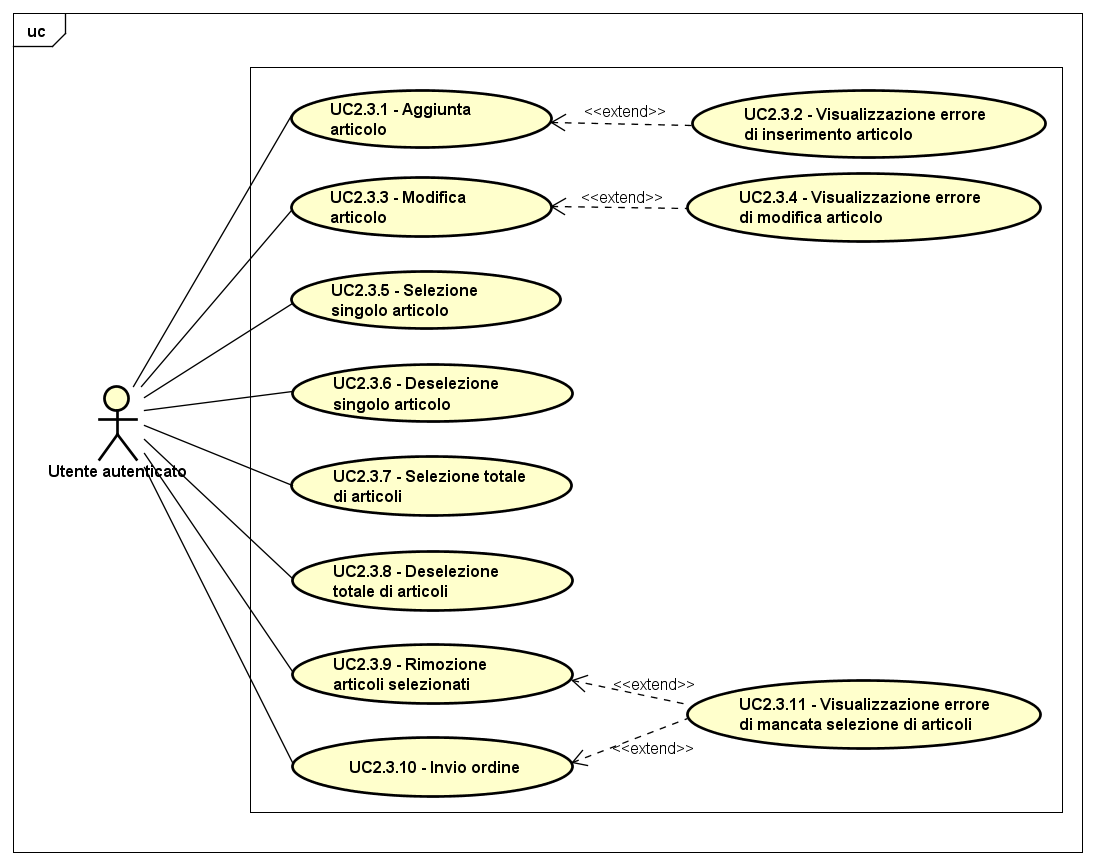
\includegraphics[width=0.9\columnwidth]{usecase/gestioneCarrello} 
    \caption{Use Case - UC1: Azioni utente non autenticato}
\end{figure}

\begin{itemize}
	\item \textbf{Attore}: Utente autenticato;
	\item \textbf{Descrizione}: L'attore può:
		\begin{enumerate}
			\item aggiungere un articolo al carrello;
			\item modificare un articolo in carrello;
			\item selezionare un singolo articolo in carrello;
			\item deselezionare un singolo articolo in carrello;
			\item selezionare tutti gli articoli in carrello;
			\item deselezionare tutti gli articoli in carrello;
			\item rimuovere articoli dal carrello;
			\item inviare un ordine.
		\end{enumerate}
	\item \textbf{Pre-condizioni}: L'attore ha avviato l'applicazione ed è riconosciuto dal sistema;
	\item \textbf{Post-condizioni}: L'attore ha eseguito le operazioni che desiderava compiere sul proprio carrello;
	\item \textbf{Scenario principale}:
		\begin{enumerate}
			\item UC2.3.1 - Aggiunta articolo;
			\item UC2.3.3 - Modifica articolo;
			\item UC2.3.5 - Selezione singolo articolo;
			\item UC2.3.6 - Deselezione singolo articolo;
			\item UC2.3.7 - Selezione totale di articoli;
			\item UC2.3.8 - Deselezione totale di articoli;
			\item UC2.3.9 - Rimozione articoli selezionati;
			\item UC2.3.10 - Invio ordine.
		\end{enumerate}
	\item \textbf{Scenari alternativi}:
		\begin{itemize}
			\item Durante l'operazione di aggiunta articolo, l'attore ha inserito un codice articolo non corrispondente a nessun articolo venduto dall'azienda, oppure ha inserito una quantità non permessa per l'articolo, oppure la scansione del codice a barre per la ricerca del codice articolo è fallita: UC2.3.2 - Visualizzazione errore di inserimento articolo;
			\item Durante l'operazione di modifica articolo, l'attore ha inserito una quantità non permessa per l'articolo: UC2.3.4 - Visualizzazione errore di modifica articolo;
			\item L'attore ha premuto il bottone di rimozione articoli selezionati senza aver selezionato alcun articolo dal carrello: UC2.3.11 - Visualizzazione errore di mancata selezione di articoli;
			\item L'attore ha premuto il bottone di invio ordine senza aver selezionato alcun articolo dal carrello: UC2.3.12 - Visualizzazione errore di mancata selezione di articoli.
		\end{itemize}
\end{itemize}

\subsection{UC2.3.1 - Aggiunta articolo}

\begin{figure}[!h] 
    \centering 
    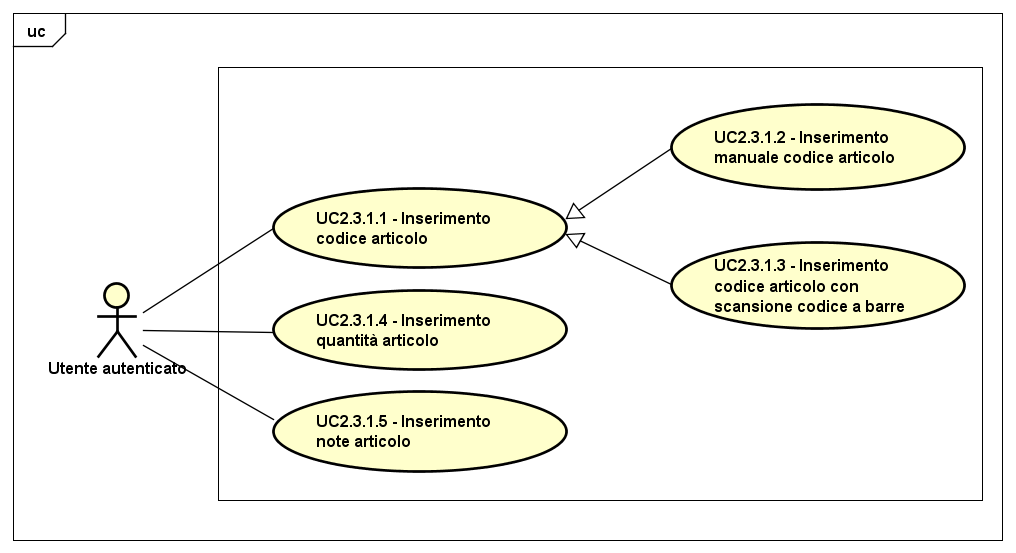
\includegraphics[width=0.9\columnwidth]{usecase/dettaglioAggiunta} 
    \caption{Use Case - UC1: Azioni utente non autenticato}
\end{figure}

\begin{itemize}
	\item \textbf{Attore}: Utente autenticato;
	\item \textbf{Descrizione}: L'attore può aggiungere un articolo al carrello;
	\item \textbf{Pre-condizioni}: L'attore ha avviato l'applicazione, è riconosciuto dal sistema e ha richiesto di aggiungere un articolo al carrello;
	\item \textbf{Post-condizioni}: L'attore ha aggiunto l'articolo al carrello;
	\item \textbf{Scenario principale}:
		\begin{enumerate}
			\item UC2.3.1.1 - Inserimento codice articolo;
			\item UC2.3.1.4 - Inserimento quantità articolo;
			\item UC2.3.1.5 - Inserimento note articolo.
		\end{enumerate}
\end{itemize}

\subsection{UC2.3.1.1 - Inserimento codice articolo}

\begin{itemize}
	\item \textbf{Attore}: Utente autenticato;
	\item \textbf{Descrizione}: L'attore deve inserire un codice articolo per l'operazione di aggiunta articolo;
	\item \textbf{Pre-condizioni}: L'attore ha avviato l'applicazione, è riconosciuto dal sistema, ha richiesto di aggiungere un articolo in carrello e il sistema richiede l'inserimento di un codice articolo per l'operazione di aggiunta articolo;
	\item \textbf{Post-condizioni}: L'attore ha inserito il codice articolo;
	\item \textbf{Scenario principale}: L'attore inserisce il codice articolo manualmente (UC2.3.1.2) o tramite la scansione di un codice a barre (UC2.3.1.3).
\end{itemize}

\subsection{UC2.3.1.2 - Inserimento manuale codice articolo}

\begin{itemize}
	\item \textbf{Attore}: Utente autenticato;
	\item \textbf{Descrizione}: L'attore deve inserire un codice articolo per l'operazione di aggiunta articolo;
	\item \textbf{Pre-condizioni}: L'attore ha avviato l'applicazione, è riconosciuto dal sistema, ha richiesto di aggiungere un articolo in carrello e quando il sistema richiede l'inserimento di un codice articolo per l'operazione di aggiunta articolo, l'attore esprime la volontà di voler inserire il codice articolo manualmente;
	\item \textbf{Post-condizioni}: L'attore ha inserito manualmente il codice articolo;
	\item \textbf{Scenario principale}: L'attore inserisce il codice articolo manualmente tramite una text box.
\end{itemize}

\subsection{UC2.3.1.3 - Inserimento codice articolo con scansione codice a barre}

\begin{itemize}
	\item \textbf{Attore}: Utente autenticato;
	\item \textbf{Descrizione}: L'attore deve inserire un codice articolo per l'operazione di aggiunta articolo;
	\item \textbf{Pre-condizioni}: L'attore ha avviato l'applicazione, è riconosciuto dal sistema, ha richiesto di aggiungere un articolo in carrello e quando il sistema richiede l'inserimento di un codice articolo per l'operazione di aggiunta articolo, l'attore esprime la volontà di voler inserire il codice articolo mediante la scansione del codice a barre di un articolo;
	\item \textbf{Post-condizioni}: L'attore ha inserito il codice articolo mediante la scansione del codice a barre dell'articolo;
	\item \textbf{Scenario principale}: L'attore inserisce il codice articolo mediante la scansione del codice a barre dell'articolo.
\end{itemize}

\subsection{UC2.3.1.4 - Inserimento quantità articolo}

\begin{itemize}
	\item \textbf{Attore}: Utente autenticato;
	\item \textbf{Descrizione}: L'attore deve inserire una quantità per l'operazione di aggiunta articolo;
	\item \textbf{Pre-condizioni}: L'attore ha avviato l'applicazione, è riconosciuto dal sistema, ha richiesto di aggiungere un articolo in carrello e il sistema richiede l'inserimento di una quantità per l'operazione di aggiunta articolo;
	\item \textbf{Post-condizioni}: L'attore ha inserito la quantità dell'articolo;
	\item \textbf{Scenario principale}: L'attore inserisce la quantità dell'articolo tramite una text box.
\end{itemize}

\subsection{UC2.3.1.5 - Inserimento note articolo}

\begin{itemize}
	\item \textbf{Attore}: Utente autenticato;
	\item \textbf{Descrizione}: L'attore può inserire delle note durante l'operazione di aggiunta articolo;
	\item \textbf{Pre-condizioni}: L'attore ha avviato l'applicazione, è riconosciuto dal sistema, ha richiesto di aggiungere un articolo in carrello e il sistema permette l'inserimento di note durante l'operazione di aggiunta articolo;
	\item \textbf{Post-condizioni}: L'attore ha inserito delle note per l'articolo;
	\item \textbf{Scenario principale}: L'attore inserisce delle note per l'articolo tramite una text area.
\end{itemize}

\subsection{UC2.3.2 - Visualizzazione errore di inserimento articolo}

\begin{itemize}
	\item \textbf{Attore}: Utente autenticato;
	\item \textbf{Descrizione}: L'attore inserisce un codice articolo non corrispondente a nessun articolo venduto dall'azienda, oppure inserisce una quantità non permessa per l'articolo, oppure la scansione del codice a barre per la ricerca del codice articolo è fallita;
	\item \textbf{Pre-condizioni}: L'attore ha avviato l'applicazione, è riconosciuto dal sistema, ha richiesto di aggiungere un articolo in carrello e ha inserito un codice articolo che non corrisponde a nessun articolo venduto dall'azienda, oppure ha inserito una quantità non permessa per l'articolo, oppure la scansione del codice a barre per la ricerca del codice articolo è fallita;
	\item \textbf{Post-condizioni}: L'attore ha visualizzato un messaggio d'errore relativo all'impossibilità di aggiungere l'articolo in carrello;
	\item \textbf{Scenario principale}: L'attore visualizza un messaggio d'errore relativo all'impossibilità di aggiungere l'articolo in carrello.
\end{itemize}

\subsection{UC2.3.3 - Modifica articolo}

\begin{figure}[!h] 
    \centering 
    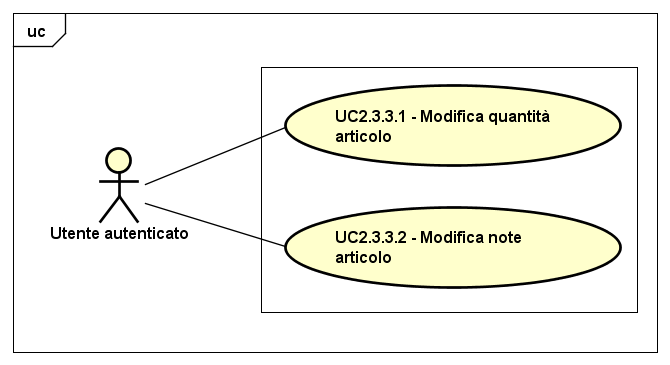
\includegraphics[width=0.9\columnwidth]{usecase/dettaglioModifica} 
    \caption{Use Case - UC1: Azioni utente non autenticato}
\end{figure}

\begin{itemize}
	\item \textbf{Attore}: Utente autenticato;
	\item \textbf{Descrizione}: L'attore può modificare un articolo in carrello;
	\item \textbf{Pre-condizioni}: L'attore ha avviato l'applicazione, è riconosciuto dal sistema e ha richiesto di modificare un articolo in carrello;
	\item \textbf{Post-condizioni}: L'attore ha modificato l'articolo in carrello;
	\item \textbf{Scenario principale}:
		\begin{enumerate}
			\item UC2.3.3.1 - Modifica quantità articolo;
			\item UC2.3.3.2 - Modifica note articolo.
		\end{enumerate}
\end{itemize}

\subsection{UC2.3.3.1 - Modifica quantità articolo}

\begin{itemize}
	\item \textbf{Attore}: Utente autenticato;
	\item \textbf{Descrizione}: L'attore può modificare la quantità dell'articolo selezionato;
	\item \textbf{Pre-condizioni}: L'attore ha avviato l'applicazione, è riconosciuto dal sistema, ha richiesto di modificare un articolo in carrello e il sistema permette la modifica della quantità dell'articolo selezionato;
	\item \textbf{Post-condizioni}: L'attore ha modificato la quantità dell'articolo selezionato;
	\item \textbf{Scenario principale}: L'attore modifica la quantità dell'articolo selezionato tramite una text box.
\end{itemize}

\subsection{UC2.3.3.2 - Modifica note articolo}

\begin{itemize}
	\item \textbf{Attore}: Utente autenticato;
	\item \textbf{Descrizione}: L'attore può modificare le note dell'articolo selezionato;
	\item \textbf{Pre-condizioni}: L'attore ha avviato l'applicazione, è riconosciuto dal sistema, ha richiesto di modificare un articolo in carrello e il sistema permette la modifica della note dell'articolo selezionato;
	\item \textbf{Post-condizioni}: L'attore ha modificato le note dell'articolo selezionato;
	\item \textbf{Scenario principale}: L'attore modifica le note dell'articolo selezionato tramite una text box.
\end{itemize}

\subsection{UC2.3.4 - Visualizzazione errore di modifica articolo}

\begin{itemize}
	\item \textbf{Attore}: Utente autenticato;
	\item \textbf{Descrizione}: L'attore inserisce una quantità non permessa per l'articolo selezionato;
	\item \textbf{Pre-condizioni}: L'attore ha avviato l'applicazione, è riconosciuto dal sistema, ha richiesto di modificare un articolo in carrello e ha inserito una quantità non permessa per l'articolo selezionato;
	\item \textbf{Post-condizioni}: L'attore ha visualizzato un messaggio d'errore relativo all'impossibilità di modificare l'articolo selezionato;
	\item \textbf{Scenario principale}: L'attore visualizza un messaggio d'errore relativo all'impossibilità di modificare l'articolo selezionato.
\end{itemize}

\subsection{UC2.3.5 - Selezione singolo articolo}

\begin{itemize}
	\item \textbf{Attore}: Utente autenticato;
	\item \textbf{Descrizione}: L'attore può selezionare un articolo non ancora selezionato in carrello;
	\item \textbf{Pre-condizioni}: L'attore ha avviato l'applicazione, è riconosciuto dal sistema e ha richiesto di selezionare un articolo non ancora selezionato in carrello;
	\item \textbf{Post-condizioni}: L'attore ha selezionato l'articolo in carrello;
	\item \textbf{Scenario principale}: L'attore seleziona l'articolo in carrello tramite una check-box.
\end{itemize}

\subsection{UC2.3.6 - Deselezione singolo articolo}

\begin{itemize}
	\item \textbf{Attore}: Utente autenticato;
	\item \textbf{Descrizione}: L'attore può deselezionare un articolo selezionato in carrello;
	\item \textbf{Pre-condizioni}: L'attore ha avviato l'applicazione, è riconosciuto dal sistema e ha richiesto di deselezionare un articolo selezionato in carrello;
	\item \textbf{Post-condizioni}: L'attore ha deselezionato l'articolo in carrello;
	\item \textbf{Scenario principale}: L'attore deseleziona l'articolo in carrello tramite una check-box.
\end{itemize}

\subsection{UC2.3.7 - Selezione totale di articoli}

\begin{itemize}
	\item \textbf{Attore}: Utente autenticato;
	\item \textbf{Descrizione}: L'attore può selezionare tutti gli articoli in carrello non ancora selezionati;
	\item \textbf{Pre-condizioni}: L'attore ha avviato l'applicazione, è riconosciuto dal sistema e ha richiesto di selezionare tutti gli articoli in carrello non ancora selezionati;
	\item \textbf{Post-condizioni}: L'attore ha selezionato tutti gli articoli in carrello non ancora selezionati;
	\item \textbf{Scenario principale}: L'attore seleziona tutti gli articoli in carrello non ancora selezionati premendo su un bottone.
\end{itemize}

\subsection{UC2.3.8 - Deselezione totale di articoli}

\begin{itemize}
	\item \textbf{Attore}: Utente autenticato;
	\item \textbf{Descrizione}: L'attore può deselezionare tutti gli articoli in carrello;
	\item \textbf{Pre-condizioni}: L'attore ha avviato l'applicazione, è riconosciuto dal sistema e ha richiesto di deselezionare tutti gli articoli in carrello;
	\item \textbf{Post-condizioni}: L'attore ha deselezionato tutti gli articoli in carrello;
	\item \textbf{Scenario principale}: L'attore deseleziona tutti gli articoli in carrello premendo su un bottone.
\end{itemize}

\subsection{UC2.3.9 - Rimozione articoli selezionati}

\begin{itemize}
	\item \textbf{Attore}: Utente autenticato;
	\item \textbf{Descrizione}: L'attore può rimuovere gli articoli selezionati dal carrello;
	\item \textbf{Pre-condizioni}: L'attore ha avviato l'applicazione, è riconosciuto dal sistema e ha richiesto di rimuovere gli articoli selezionati dal carrello;
	\item \textbf{Post-condizioni}: L'attore ha rimosso gli articoli selezionati dal carrello;
	\item \textbf{Scenario principale}: L'attore rimuove gli articoli selezionati dal carrello premendo su un bottone.
\end{itemize}

\subsection{UC2.3.10 - Invio ordine}

\begin{figure}[!h] 
    \centering 
    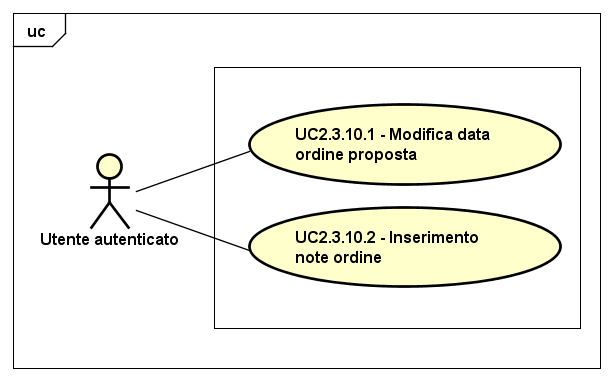
\includegraphics[width=0.9\columnwidth]{usecase/dettaglioInvioOrdine} 
    \caption{Use Case - UC1: Azioni utente non autenticato}
\end{figure}

\begin{itemize}
	\item \textbf{Attore}: Utente autenticato;
	\item \textbf{Descrizione}: L'attore può inviare un ordine composto dagli articoli selezionati in carrello;
	\item \textbf{Pre-condizioni}: L'attore ha avviato l'applicazione, è riconosciuto dal sistema e ha richiesto di inviare un ordine composto dagli articoli selezionati in carrello;
	\item \textbf{Post-condizioni}: L'attore ha inviato un ordine composto dagli articoli selezionati in carrello;
	\item \textbf{Scenario principale}:
		\begin{enumerate}
			\item UC2.3.10.1 - Modifica data ordine proposta;
			\item UC2.3.10.2 - Inserimento note ordine.
		\end{enumerate}
\end{itemize}

\subsection{UC2.3.10.1 - Modifica data ordine proposta}

\begin{itemize}
	\item \textbf{Attore}: Utente autenticato;
	\item \textbf{Descrizione}: L'attore può modificare la data d'ordine proposta;
	\item \textbf{Pre-condizioni}: L'attore ha avviato l'applicazione, è riconosciuto dal sistema, ha richiesto di inviare un ordine e il sistema permette la modifica della data d'ordine proposta;
	\item \textbf{Post-condizioni}: L'attore ha modificato la data d'ordine proposta;
	\item \textbf{Scenario principale}: L'attore modifica la data d'ordine proposta tramite una text box.
\end{itemize}

\subsection{UC2.3.10.2 - Inserimento note ordine}

\begin{itemize}
	\item \textbf{Attore}: Utente autenticato;
	\item \textbf{Descrizione}: L'attore può delle note per l'ordine;
	\item \textbf{Pre-condizioni}: L'attore ha avviato l'applicazione, è riconosciuto dal sistema, ha richiesto di inviare un ordine e il sistema permette l'inserimento di note per l'ordine;
	\item \textbf{Post-condizioni}: L'attore ha inserito le note per l'ordine;
	\item \textbf{Scenario principale}: L'attore le note per l'ordine tramite una text area.
\end{itemize}

\subsection{UC2.3.11 - Visualizzazione errore di mancata selezione di articoli}

\begin{itemize}
	\item \textbf{Attore}: Utente autenticato;
	\item \textbf{Descrizione}: L'attore preme sul bottone di rimozione articoli o invio ordine senza aver selezionato degli articoli in carrello;
	\item \textbf{Pre-condizioni}: L'attore ha avviato l'applicazione, è riconosciuto dal sistema, ha richiesto di rimuovere degli articoli dal carrello o di inviare un ordine, senza aver effettivamente selezionato degli articoli in carrello;
	\item \textbf{Post-condizioni}: L'attore ha visualizzato un messaggio d'errore relativo all'impossibilità di rimuovere gli articoli selezionati o inviare un ordine composto dagli articoli selezionati;
	\item \textbf{Scenario principale}: L'attore visualizza un messaggio d'errore relativo all'impossibilità di rimuovere gli articoli selezionati o inviare un ordine composto dagli articoli selezionati.
\end{itemize}

\section{Requisiti}

In questa sezione sono presentati i requisiti della piattaforma moviORDER, dedotti dai diagrammi dei casi d'uso, dall'analisi preliminare fornita dal tutor aziendale e da raffinamenti di questa, ottenuti in seguito a brevi interazioni avvenute con il tutor aziendale. I requisiti sono stati classificati dallo stagista in base alla loro tipologia e importanza strategica. Sono stati individuati:
\begin{enumerate}
	\item \textbf{requisiti funzionali}: descrivono funzionalità del sistema;
	\item \textbf{requisiti qualitativi}: descrivono qualità del prodotto finale;
	\item \textbf{requisiti di vincolo}: descrivono vincoli imposti dal tutor aziendale o dal dominio del problema.
\end{enumerate}

L'importanza strategica dei requisiti individuati è stata negoziata con il tutor aziendale e si è deciso che ciascun requisito deve appartenere ad una delle seguenti categorie:
\begin{itemize}
	\item \textbf{obbligatorio}: non più negoziabile e irrinunciabile per il tutor aziendale;
	\item \textbf{desiderabile}: rappresenta un valore aggiunto d'interesse riconosciuto da parte del tutor aziendale;
	\item \textbf{facoltativo}: relativamente utile per gli scopi dell'applicazione.
\end{itemize}

Nelle seguenti sezioni vengono dettagliati i requisiti di moviORDER. In ogni sezione è presente una tabella contenente per ogni requisito:
\begin{itemize}
	\item \textbf{codice identificativo}: codice che identifica univocamente il requisito, a fini di tracciabilità;
	\item \textbf{descrizione}: breve descrizione testuale del requisito;
	\item \textbf{fonte}: fonte da cui è stato dedotto il requisito, sempre a fini di tracciabilità.
\end{itemize}

\newpage

\subsection{Requisiti funzionali}

\begin{table}%
\caption{Tabella del tracciamento dei requisti funzionali}
\label{tab:requisiti-funzionali}
\begin{tabularx}{\textwidth}{lXl}
\hline\hline
\textbf{Requisito} & \textbf{Descrizione} & \textbf{Fonte}\\
\hline
RFO & Se l'applicazione viene lanciata in assenza di connettività, deve essere visualizzato un messaggio d'errore di connettività assente e l'applicazione deve essere chiusa & UC \\
RFO1 & L'utente non autenticato deve poter accedere all'applicazione & UC1.1 \\
RFO1.1 & Per accedere, l'utente non autenticato deve poter inserire una username & UC1.1.1 \\
RFO1.2 & Per accedere, l'utente non autenticato deve poter inserire una password & UC1.1.2 \\
RFO & L'utente autenticato deve poter tentare l'accesso premendo su un bottone di login & \\
RFO & Se l'utente non autenticato inserisce una username non esistente e preme sul bottone di login, deve essere visualizzato un messaggio d'errore di username inesistente & UC \\
RFO & Se l'utente non autenticato inserisce una password non corrispondente alla username inserita e preme sul bottone di login, deve essere visualizzato un messaggio d'errore di password errata & UC \\
RFO & Se l'utente non autenticato preme sul bottone di login senza aver inserito le credenziali di accesso, deve essere visualizzato un messaggio che inviti l'utente ad inserire delle credenziali & UC \\
RFO & Se il server non risponde in fase di login, deve essere visualizzato un messaggio d'errore che notifichi che il server è down & UC \\
RFO & Se l'utente non autenticato riesce ad accedere, deve essere visualizzata la home page dell'applicazione & UC \\
RFO & L'utente autenticato deve visualizzare la propria ragione sociale nella home page & UC \\
RFO & L'utente autenticato deve poter visualizzare il tutorial dell'applicazione nella home page & UC \\
RFO & L'utente autenticato deve poter effettuare il logout dall'applicazione premendo su un bottone sulla home page& UC \\
RFO & L'utente autenticato deve poter visualizzare i propri articoli nel carrello nella home page & UC \\
RFO & Se l'utente autenticato non presenta articoli in carrello deve essere visualizzata una frase che notifichi che il carrello è vuoto & UC \\
RFO & La visualizzazione di un articolo in carrello deve comprendere una check-box per la selezione dell'articolo & UC \\
RFO & La visualizzazione di un articolo in carrello deve comprendere la quantità dell'articolo & UC \\
RFO & La visualizzazione di un articolo in carrello deve comprendere il codice dell'articolo & UC \\
RFO & La visualizzazione di un articolo in carrello deve comprendere la descrizione dell'articolo & UC \\
RFO & L'utente autenticato deve poter aggiungere un nuovo articolo al carrello dalla home page & UC \\
RFO & Per aggiungere un nuovo articolo al carrello, l'utente autenticato deve inserire un codice articolo & UC \\
RFO & L'utente autenticato deve poter decidere se inserire il codice articolo con la scansione di un codice a barre o manualmente & UC \\
RFO & Se l'utente autenticato decide di inserire il codice articolo con la scansione di un codice a barre, l'applicazione deve accedere alla fotocamera e permettere la cattura del codice a barre & UC \\
RFO & L'applicazione deve permettere la cattura del codice a barre di tipo ... & UC \\
RFO & L'utente autenticato deve poter annullare la scansione del codice a barre con il tasto indietro & UC \\
RFO & Se l'utente autenticato annulla la scansione del codice a barre deve essere visualizzato un messaggio di annullamento della scansione da parte dell'utente & UC \\
RFO & Se la scansione del codice a barre fallisce, la fotocamera deve essere chiusa e deve essere visualizzato un messaggio d'errore di scansione fallita & UC \\
RFO & Se la scansione del codice a barre va a buon fine ma il codice ottenuto non corrisponde ad un articolo venduto dall'azienda deve essere visualizzato un messaggio d'errore che notifichi il problema & UC \\
RFO & Se la scansione del codice a barre va a buon fine e il codice ottenuto corrisponde ad un articolo venduto dall'azienda ma l'articolo è già presente in carrello, deve essere visualizzato un messaggio che inviti l'utente a cambiare la quantità dell'articolo in carrello & UC \\
RFO & Se la scansione del codice a barre va a buon fine e il codice ottenuto corrisponde ad un articolo venduto dall'azienda deve essere visualizzata la pagina di aggiunta articolo & UC \\
RFO & Se l'utente autenticato decide di inserire il codice articolo manualmente deve essere visualizzata una text box per l'inserimento del codice & UC \\
RFO & Se l'utente autenticato inserisce un codice articolo che non corrisponde ad un articolo venduto dall'azienda, deve essere visualizzato un messaggio d'errore che notifichi il problema & UC \\
RFO & Se l'utente autenticato inserisce un codice articolo che corrisponde ad un articolo venduto dall'azienda ma l'articolo è già presente in carrello, deve essere visualizzato un messaggio che inviti l'utente a cambiare la quantità dell'articolo in carrello & UC \\
RFO & Se l'utente autenticato inserisce un codice articolo che corrisponde ad un articolo venduto dall'azienda, deve essere visualizzata la pagina di aggiunta articolo & UC \\
RFO & L'utente autenticato deve poter visualizzare il codice articolo nella pagina di aggiunta articolo & UC \\
RFO & L'utente autenticato deve poter visualizzare la descrizione dell'articolo nella pagina di aggiunta articolo & UC \\
RFO & L'utente autenticato deve poter visualizzare le informazioni dell'articolo nella pagina di aggiunta articolo & UC \\
RFO & La pagina di aggiunta articolo deve proporre all'utente autenticato una quantità minima per l'articolo da ordinare & UC \\
RFO & L'utente autenticato deve poter inserire una quantità per l'articolo da ordinare nella pagina di aggiunta articolo & UC \\
RFO & L'utente autenticato deve poter inserire delle note per l'articolo da ordine nella pagina di aggiunta articolo & \\
RFO & L'utente autenticato deve poter annullare l'inserimento dell'articolo nella pagina di aggiunta articolo & \\
RFO & L'utente autenticato deve poter confermare l'inserimento dell'articolo nella pagina di aggiunta articolo & \\
RFO & Se l'utente autenticato conferma l'inserimento dell'articolo ed ha inserito una quantità errata (troppo bassa, troppo alta o che non soddisfa uno step impostato dall'azienda) deve essere visualizzato un messaggio d'errore di errata quantità inserita & \\
RFO & Se l'utente autenticato conferma l'inserimento dell'articolo e i dati inseriti sono corretti, deve essere visualizzata la home page e il nuovo articolo deve essere presente in carrello & \\
RFO & Se l'utente autenticato annulla l'inserimento dell'articolo, deve essere visualizzata la home page e il carrello non deve essere cambiato & \\
RFO & L'utente autenticato deve poter selezionare un articolo in carrello premendo sulla relativa check-box & \\
RFO & L'utente autenticato deve poter deselezionare un articolo in carrello selezionato premendo sulla relativa check-box & \\
RFO & L'utente autenticato deve poter selezionare tutti gli articoli in carrello premendo su un bottone di seleziona tutti/deseleziona tutti presente nella home page & \\
RFO & L'utente autenticato deve poter deselezionare tutti gli articoli in carrello premendo su un bottone di seleziona tutti/deseleziona tutti presente nella home page & \\
RFO & L'utente autenticato deve poter modificare un articolo in carrello premendo sopra l'articolo direttamente sul carrello & \\
RFO & Se l'utente autenticato preme su un articolo in carrello deve essere visualizzato un dialog che chiede all'utente se vuole modificare l'articolo & \\
RFO & Se l'utente autenticato accetta di modificare l'articolo sul dialog di conferma, deve essere aperta la pagina di modifica articolo & \\
RFO & Se l'utente autenticato rifiuta di modificare l'articolo sul dialog di conferma, deve essere visualizzata la home page senza cambiamenti sul carrello & \\
RFO & L'utente autenticato deve poter visualizzare il codice articolo dell'articolo selezionato nella pagina di modifica articolo & UC \\
RFO & L'utente autenticato deve poter visualizzare la descrizione dell'articolo dell'articolo selezionato nella pagina di modifica articolo & UC \\
RFO & L'utente autenticato deve poter visualizzare le informazioni dell'articolo dell'articolo selezionato nella pagina di modifica articolo & UC \\
RFO & La pagina di modifica articolo deve proporre all'utente autenticato la quantità precedentemente inserita per l'articolo selezionato & UC \\
RFO & L'utente autenticato deve poter cambiare la quantità per l'articolo selezionato nella pagina di modifica articolo & UC \\
RFO & La pagina di modifica articolo deve proporre all'utente autenticato le note precedentemente inserite per l'articolo selezionato & UC \\
RFO & L'utente autenticato deve poter modificare le note per l'articolo selezionato nella pagina di modifica articolo & \\
RFO & L'utente autenticato deve poter annullare la modifica dell'articolo nella pagina di modifica articolo & \\
RFO & L'utente autenticato deve poter confermare la modifica dell'articolo nella pagina di modifica articolo & \\
RFO & Se l'utente autenticato conferma la modifica dell'articolo ed ha inserito una quantità errata (troppo bassa, troppo alta o che non soddisfa uno step impostato dall'azienda) deve essere visualizzato un messaggio d'errore di errata quantità inserita & \\
RFO & Se l'utente autenticato conferma la modifica dell'articolo e i dati modificati sono corretti, deve essere visualizzata la home page e l'articolo modificato deve essere presente in carrello con le modifiche apportate & \\
RFO & Se l'utente autenticato annulla la modifica dell'articolo, deve essere visualizzata la home page e l'articolo selezionato non deve essere stato modificato & \\
RFO & L'utente autenticato deve poter rimuovere gli articoli selezionati sul carrello premendo su un bottone presente sulla home page & \\
RFO & Se l'utente autenticato preme sul bottone di rimozione articoli senza aver selezionato alcun articolo, deve essere visualizzato un messaggio che inviti l'utente a selezionare degli articoli & \\
RFO & Se l'utente autenticato preme sul bottone di rimozione articoli avendo selezionato degli articoli sul carrello deve essere richiesta la conferma di eliminazione tramite un dialog & \\
RFO & Se l'utente autenticato conferma l'eliminazione sul dialog di conferma, gli articoli precedentemente selezionati devono essere rimossi dal carrello & \\
RFO & Se l'utente autenticato rifiuta l'eliminazione sul dialog di conferma, il carrello non deve subire cambiamenti & \\
RFO & L'utente autenticato deve poter inviare un ordine composto dagli articoli selezionati sul carrello premendo su un bottone di invio ordine & \\
RFO & Se l'utente autenticato preme sul bottone di invio ordine senza aver selezionato alcun articolo, deve essere visualizzato un messaggio che inviti l'utente a selezionare degli articoli & \\
RFO & Se l'utente autenticato preme sul bottone di invio ordine avendo selezionato degli articoli sul carrello deve essere visualizzato il modal di invio ordine & \\
RFO & L'utente autenticato deve poter visualizzare il codice cliente nel modal di invio ordine & \\
RFO & L'utente autenticato deve poter visualizzare la descrizione cliente nel modal di invio ordine & \\
RFO & L'utente autenticato deve poter visualizzare il codice del documento da generare per l'ordine nel modal di invio ordine & \\
RFO & L'utente autenticato deve poter visualizzare la descrizione del documento da generare per l'ordine nel modal di invio ordine & \\
RFO & Il modal di invio ordine deve proporre all'utente autenticato la data corrente come data d'ordine & \\
RFO & L'utente autenticato deve poter modificare la data d'ordine proposta nel modal di invio ordine & \\
RFO & L'utente autenticato deve poter inserire delle note per l'ordine nel modal di invio ordine & \\
RFO & L'utente autenticato deve poter confermare l'invio dell'ordine nel modal di invio ordine & \\
RFO & L'utente autenticato deve poter annullare l'invio dell'ordine nel modal di invio ordine & \\
RFO & Se l'utente autenticato decide di annullare l'invio dell'ordine, il modal di invio ordine deve essere chiuso & \\
RFO & Se l'utente autenticato decide di confermare l'invio dell'ordine, deve essere richiesta la conferma di invio ordine tramite un dialog & \\
RFO & Se l'utente autenticato conferma l'invio dell'ordine nel dialog di conferma e l'ordine è andato a buon fine, deve essere visualizzato un messaggio di ordine inviato con successo e una mail di conferma deve essere inviata sia all'utente che all'azienda & \\
RFO & Se l'utente autenticato conferma l'invio dell'ordine nel dialog di conferma e l'ordine non è andato a buon fine, deve essere visualizzato un messaggio d'errore di mancato invio dell'ordine & \\
RFO & Se l'utente autenticato annulla l'invio dell'ordine nel dialog di conferma, il dialog di conferma deve essere chiuso & \\
RFO & Se viene persa la connettività nella home page, deve essere visualizzato un messaggio che invita l'utente a chiudere l'applicazione per connettività assente & \\
RFO & Se viene persa la connettività nella pagina di aggiunta articolo, deve essere visualizzato un messaggio che invita l'utente a chiudere l'applicazione per connettività assente & \\
RFO & Se viene persa la connettività nella pagina di modifica, deve essere visualizzato un messaggio che invita l'utente a chiudere l'applicazione per connettività assente & \\
RFO & La mail inviata dal sistema al momento dell'invio dell'ordine deve contenere in oggetto la data di registrazione dell'ordine & \\
RFO & La mail inviata dal sistema al momento dell'invio dell'ordine deve contenere in oggetto il codice azienda dell'utente che ha effettuato l'ordine & \\
RFO & La mail inviata dal sistema al momento dell'invio dell'ordine deve contenere in oggetto la tipologia di documento generato con l'ordine & \\
RFO & La mail inviata dal sistema al momento dell'invio dell'ordine deve contenere nel corpo il codice cliente del cliente che ha effettuato l'ordine & \\
RFO & La mail inviata dal sistema al momento dell'invio dell'ordine deve contenere nel corpo una tabella contenente i dati degli articoli inviati & \\
RFO & Per ogni articolo in tabella deve essere indicata la quantità ordinata & \\
RFO & Per ogni articolo in tabella deve essere indicato il codice articolo & \\
RFO & Per ogni articolo in tabella deve essere indicata la descrizione dell'articolo & \\
RFO & RFO & La mail inviata dal sistema al momento dell'invio dell'ordine deve contenere nel corpo l'avviso di non rispondere alla mail & \\
RFO &  & \\
RFO &  & \\
RFO &  & \\
RFO &  & \\
RFO &  & \\
RFO &  & \\
RFO &  & \\
RFO &  & \\
RFO &  & \\
RFO &  & \\
RFO &  & \\
RFO &  & \\
RFO &  & \\
RFO &  & \\
RFO &  & \\
RFO &  & \\
RFO &  & \\
RFO &  & \\
RFO &  & \\
RFO &  & \\
RFO &  & \\
RFO &  & \\
RFO &  & \\
RFO &  & \\
RFO &  & \\
RFO &  & \\
RFO &  & \\
RFO &  & \\
RFO &  & \\
RFO &  & \\
RFO &  & \\
RFO &  & \\
RFO &  & \\
RFO &  & \\
RFO &  & \\
RFO &  & \\
RFO &  & \\
RFO &  & \\
RFO &  & \\
RFO &  & \\
RFO &  & \\
RFO &  & \\
RFO &  & \\
RFO &  & \\
RFO &  & \\
RFO &  & \\
RFO &  & \\
RFO &  & \\
RFO &  & \\
RFO &  & \\
RFO &  & \\
RFO &  & \\
RFO &  & \\
RFO &  & \\
RFO &  & \\
RFO &  & \\
RFO &  & \\
RFO &  & \\
RFO &  & \\
RFO &  & \\
RFO &  & \\
RFO &  & \\
RFO &  & \\
RFO &  & \\
RFO &  & \\
RFO &  & \\
RFO &  & \\
RFO &  & \\
RFO &  & \\
RFO &  & \\
RFO &  & \\
RFO &  & \\
RFO &  & \\
RFO &  & \\
RFO &  & \\
RFO &  & \\
RFO &  & \\
RFO &  & \\
RFO &  & \\
RFO &  & \\
RFO &  & \\
RFO &  & \\
RFO &  & \\
RFO &  & \\
RFO &  & \\
RFO &  & \\
\hline
\end{tabularx}
\end{table}%

\subsection{Requisiti qualitativi}

\begin{table}%
\caption{Tabella del tracciamento dei requisiti qualitativi}
\label{tab:requisiti-qualitativi}
\begin{tabularx}{\textwidth}{lXl}
\hline\hline
\textbf{Requisito} & \textbf{Descrizione} & \textbf{Use Case}\\
\hline
RQD-1    & Le prestazioni del simulatore hardware deve garantire la giusta esecuzione dei test e non la generazione di falsi negativi & - \\
\hline
\end{tabularx}
\end{table}%

\subsection{Requisiti di vincolo}

\begin{table}%
\caption{Tabella del tracciamento dei requisiti di vincolo}
\label{tab:requisiti-vincolo}
\begin{tabularx}{\textwidth}{lXl}
\hline\hline
\textbf{Requisito} & \textbf{Descrizione} & \textbf{Use Case}\\
\hline
RVO-1    & La libreria per l'esecuzione dei test automatici deve essere riutilizzabile & - \\
\hline
\end{tabularx}
\end{table}%

\subsection{Validazione dei requisiti}